\documentclass{article}
\usepackage[parfill]{parskip}
\usepackage[absolute]{textpos}
\usepackage{graphicx}
\usepackage[T1]{fontenc}
\usepackage[scaled]{helvet}
\usepackage[final]{pdfpages}
%\usepackage[scaled]{helvet}

\usepackage{lscape}
\usepackage{courier}
\renewcommand*\familydefault{\sfdefault}
\usepackage[left=1in,top=1in,bottom=1.25in,right=1in]{geometry}
\usepackage{color}
\usepackage{fancyhdr,lastpage}
\pagestyle{fancy}
\rhead{\scriptsize \opnum:  \optitle}
%\chead{Middle top}
\newenvironment{changemargin}[2]{%
\begin{list}{}{%
\setlength{\topsep}{0pt}%
\setlength{\leftmargin}{#1}%
\setlength{\rightmargin}{#2}%
\setlength{\listparindent}{\parindent}%
\setlength{\itemindent}{\parindent}%
\setlength{\parsep}{\parskip}%
}%
\item[]}{\end{list}}
\lhead{
\includegraphics[scale=.6]{logonew.pdf}\\\smallskip\scriptsize Qualification}
\setlength{\headsep}{.75in}
\fancyfoot[C]{Page \thepage\ of \pageref{LastPage}}
\usepackage[colorlinks=true,linkcolor=black,urlcolor=blue]{hyperref}

%\newcommand{\opnum}{Release 2} 
\newcommand{\optitle}{Pharmacometrics TFL Generator Requirements}
\newcommand{\opnum}{Release 1.0.0} 
\newcommand{\tfl}{Pharmacometrics TFL Generator}

\begin{document}

\vspace*{3cm}
{\Large{\textbf{\opnum\newline \newline \optitle}}}
\vspace{3.0cm}

\begin{tabular}{p{11.0cm}p{2.0cm}}
\hline
Authored by & Date \vspace{1cm}\\

\hline
Approved by & Date \vspace{2cm}\\

\end{tabular}


\newpage
\vspace{3in}
\section*{Introduction}
The \tfl\ is a shiny application, written in R, intended to provide a graphical interface for creation of typical Tables, Figures, and Listings.  The app generates report-ready graphics, tables, and reports; but also allows for interactivity and data exploration via input from the pharamacometrics scientist.  The \tfl\ is is architected to run behind shiny-server and can handle multiple simultaneous users per application.  The application runs in a mode that assigns a new R process to each new connection, ensuring no conflicts between shared objects in the R environment. 

The application is intended to be fit for purpose of regulatory submissions, and as such has functionality to ensure reproducibility.  Upon demand, the application will create an R script that, when sourced, will duplicate any objects created from within the application.  The application also allows template loading so that a similar set of tables, figures, and listings may easily be shared between multiple users.

The functional requirements for the application are listed in the requirements traceability matrix below.
\newpage
\section*{Requirements traceability matrix}

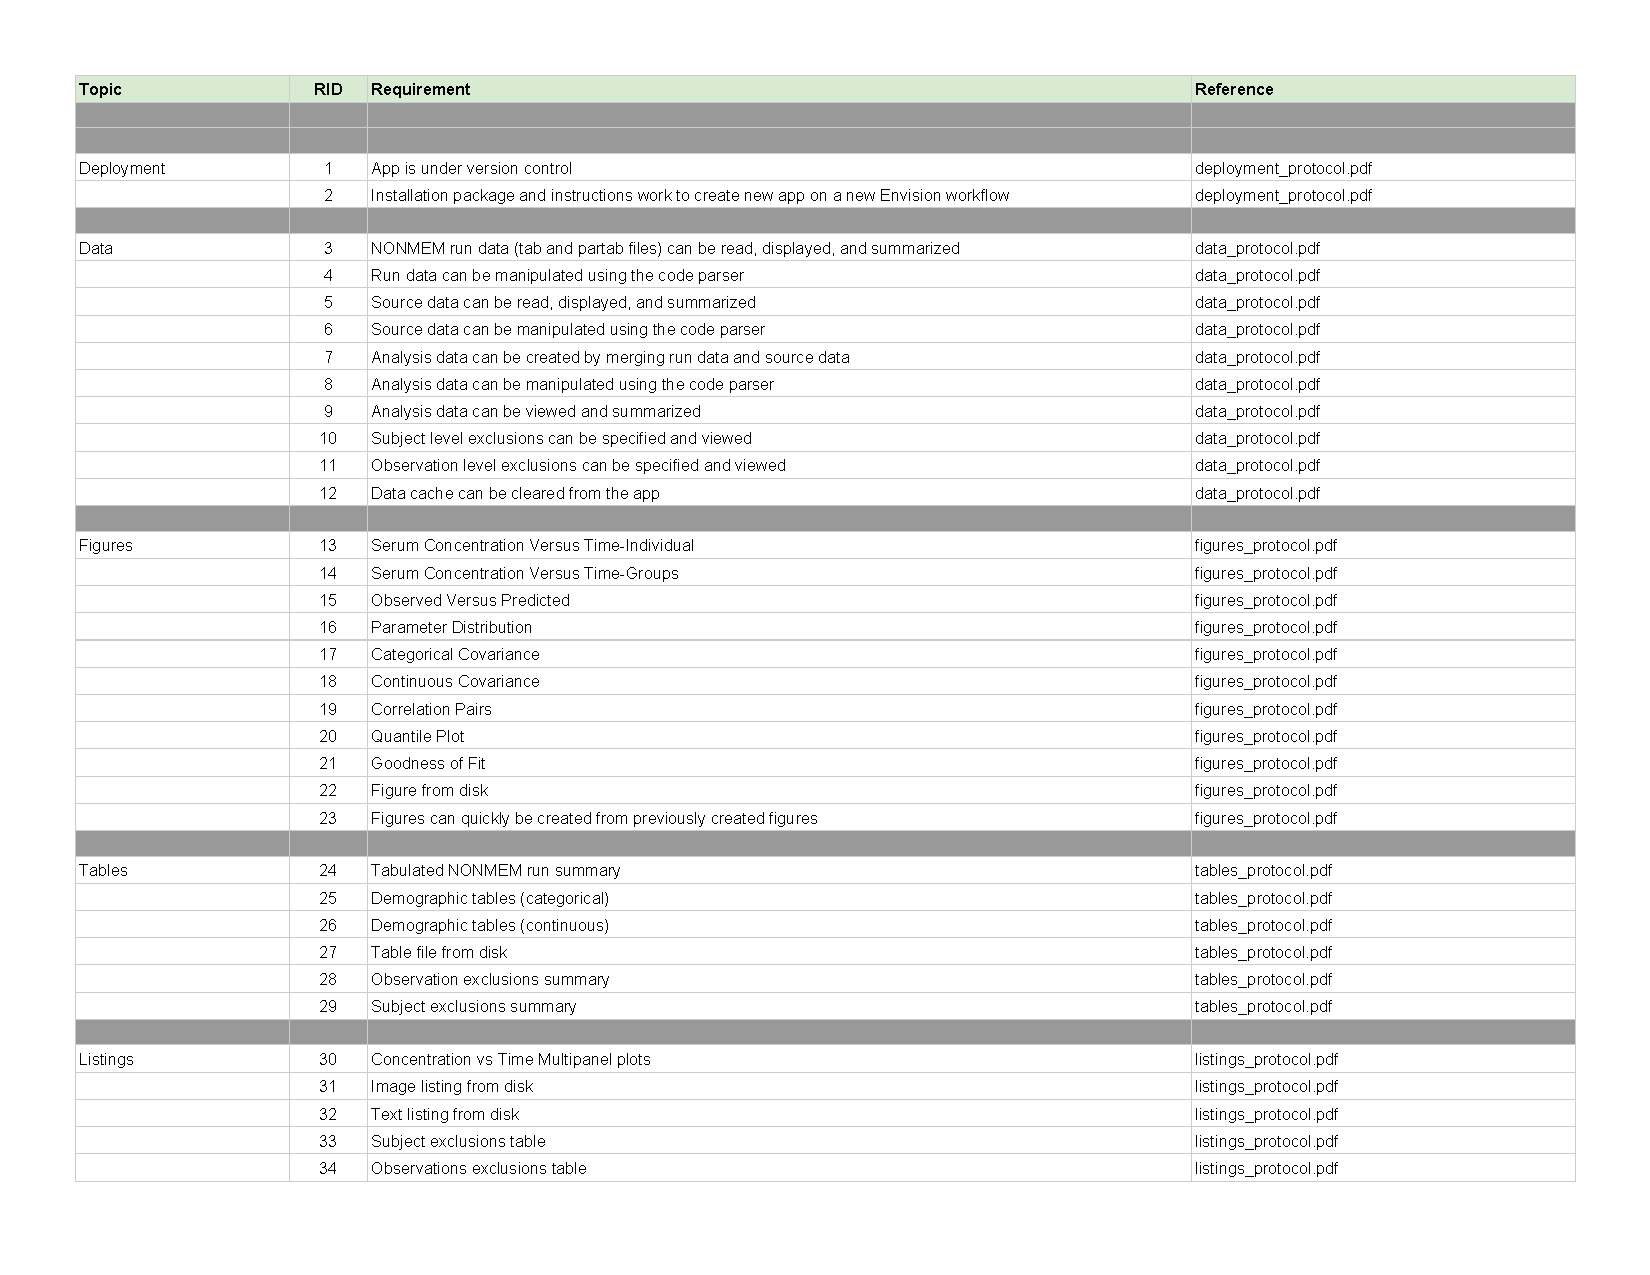
\includepdf[pages=-]{REQUIREMENTS_Pharmacometrics_TFL_generator.pdf}


\end{document}
